% !TeX root = ../main.tex
% Add the above to each chapter to make compiling the PDF easier in some editors.

\chapter{Background}\label{chapter:background}
  Abstract interpretation is the theory of approximating computer programs in a sound manner. That means that an abstraction might not be absolutely precise, but it definitely is not wrong, i.e., all possible concrete states and properties of a program are described by their abstraction.\\
  An application of abstract interpretation is static analysis. As Rival~\parencite{rival2020introduction} defines it, static analysis is "[...]an automatic technique that approximates in a conservative manner semantic properties of programs before their execution". This means that the program is analyzed just by the given source code without execution. The goal is to prove certain properties about the program in a "sound" manner, i.e., any property that is proven to hold actually does hold. However, from failing to prove a property one cannot conclude that the given property does not hold.\\
  To prove properties, e.g. finding that a program does not contain races or identifying dead code, information about the program has to be gained. This is done by performing various kinds of analyses. We will focus on flow-sensitive analyses in this thesis, i.e., analyses that find properties of the program dependent on the location within it. We will introduce a syntax to formalize flow-sensitive analyses in the following sections. This formalization approach is heavily based on \parencite{apinis2012side}.

\begin{figure}
  \centering
  \begin{subfigure}{.35\textwidth}
    \centering
    \lstinputlisting[language=C]{../code/02-example_cfg.c}
  \end{subfigure}
  \begin{subfigure}{.35\textwidth}
    \centering
    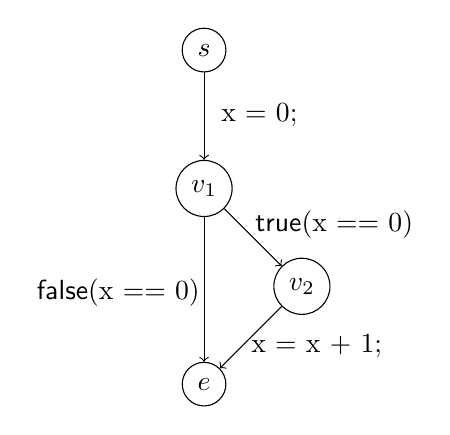
\begin{tikzpicture}[node distance={50pt}, main/.style = {draw, circle}] 
      \node[main] (0) {$s$};
      \node[main] (1) [below of=0] {$v_1$};
      \node[main] (2) [below right of=1] {$v_2$};
      \node[main] (3) [below left of=2] {$e$};
      \draw[->] (0) -- node[midway, xshift=20pt, yshift=16pt, pos=1] {x = 0;} (1);
      \draw[->] (1) -- node[midway, xshift=19pt, yshift=15pt, pos=1] {\textsf{true}(x == 0)} (2);
      \draw[->] (2) -- node[midway, xshift=35pt, yshift=8pt, pos=1] {x = x + 1;} (3);
      \draw[->] (1) -- node[midway, xshift=-31pt, yshift=25pt, pos=1] {\textsf{false}(x == 0)} (3);
    \end{tikzpicture}
  \end{subfigure}
  \caption{Example program (left) and corresponding CFG (right)}
  \label{fig:example_cfg}
\end{figure}
  
  \section{Flow sensitive analysis}
    As noted above flow sensitive analyses aim to find properties of the program dependent on the point within the program. Expressed differently this means a flow-sensitive analysis will find an overapproximation of states the program may be in for any given point within the program, from now on called "program point". This state can describe many things dependent on the analysis performed.\\
    First, we define what a program point is: Consider a CFG (Control Flow Graph), where nodes represent points between instructions within the program. Edges are labeled with instructions or checks (from now on collectively called "actions") and describe the transitions between these points (see example \autoref{fig:example_cfg}). Then any node on this CFG is what we call a program point.\\
    Concretely let $N$ be the set of all program points. Furthermore, let $\mathbb{D}$ be a domain containing abstract states describing concrete states of the program. This means that some $d \in \mathbb{D}$ can describe many states the program can be in. A concretization function $\gamma: \mathbb{D} \rightarrow 2^{\mathcal{C}}$ can be defined to extract the set of concrete states which are described by an abstract state. Here $\mathcal{C}$ is the set of all possible concrete states.\\ 
    Then an analysis is expected to find a mapping $\eta: N \rightarrow \mathbb{D}$ which maps program points to abstract states describing that location within the program, i.e., for $[v] \in N$, $\eta\ [v]$ should be an abstract state describing all possible states (and possibly more) the program can be in at program point $[v]$.\\
    \\
    As an example, we will introduce a values-of-variables analysis for integers. This analysis finds a mapping from a set of program variables $X$ to abstractions of their possible values at any given program point. Our toy language will support global variables (globals) as well as local variables (locals). The global variables can be accessed and changed by any procedure, while local ones are only visible to the procedure in which it was declared and can only be accessed and changed by this procedure. Therefore, our set $X$ of variables is the disjoint union of globals $G$ and locals $L$: $X = G \uplus L$.
    In the scope of this thesis, we will focus on abstracting integer values by sets of integers. Thereby the goal of our values-of-variables analysis is to find a mapping $X \rightarrow 2^\mathbb{N}$ for each program point.\\
    Combining this with the considerations from above, we chose the mapping $\mathbb{D}_\textsf{v} = X \rightarrow 2^\mathbb{N}$ as the abstract domain for the values-of-variables analysis. To illustrate what an abstract state from this domain describes, we define the concretization function $\gamma_\textsf{v}: \mathbb{D}_\textsf{v} \rightarrow 2^{\mathcal{C}_\textsf{v}}$. Here a concrete state is a mapping from variables to a single value each: $\mathcal{C}_\textsf{v} = X \rightarrow \mathbb{N}$. Thus, we define the concretization function as follows:
    \[ \gamma_\textsf{v}\ M = \{ \widehat{M} \in \mathcal{C}_\textsf{v} | \forall x \in X: (\widehat{M}\ x) \in (M\ x) \} \]
    In summary this the resulting $\eta_\textsf{v}: N \rightarrow \mathbb{D}_\textsf{v}$ for this analysis describes a mapping $\eta_\textsf{v}\ [v]$ for some program point $[v] \in N$, where $\eta_\textsf{v}\ [v]\ x$ is a set containing all values $x \in X$ may possibly hold at $[v]$. From this we can conclude that $x$ cannot hold any value outside $\eta_\textsf{v}\ [v]\ x$ at program point $[v]$. 

  \section{Constraint systems}
    We now formulate a way in which we can describe an analysis in the form of constraints. For this we need a partial ordering $\sqsubseteq$ on the domain $\mathbb{D}$.\\
    Then we create a system of constraints that can be solved for a solution. Consider the edges $(u, A, v)$ of the CFG, where each edge denotes a transition from program point $[u]$ to program point $[v]$ via the action $A$. Now let each of these edges give rise to a constraint
    \[\eta\ [v] \sqsupseteq [\![A]\!]^{\#}\ (\eta\ [u])\]
    where $[\![A]\!]^{\#}$ denotes the abstract effect of the action $A$ defining our analysis. In addition, we need a start state. This is given by $\textsf{init}^{\#}: \mathbb{D}$ which is defined depending on the analysis. This gives rise to the start constraint $\eta\ [s] \sqsupseteq \textsf{init}^{\#}$ for the starting point of the program $[s] \in N$.\\
    \\
    We will show these ideas with our example of the values-of-variables analysis: For this, a partial ordering $\sqsubseteq_\textsf{v}$ on the domain $\mathbb{D}$ has to be defined. This ordering is needed to formulate the constraints. We define $\sqsubseteq_\textsf{v}$ as follows: A mapping $M_1 \in \mathbb{D}_\textsf{v}$ is ordered below or equal to another mapping $M_2$, if and only if for every variable $x \in X$, the set $x$ is mapped to in $M_1$ is a subset of or equal to the one $x$ is mapped to in $M_2$. Formulated formally this is:
    \[M_1, M_2 \in \mathbb{D}_\textsf{v}: M_1 \sqsubseteq_\textsf{v} M_2 \Longleftrightarrow \forall x \in X: M_1\ x \subseteq M_2\ x\]
    Next, we define the start state $\textsf{init}^{\#} = M_\top$ for this domain as the mapping that maps every variable to the full set of integers $\mathbb{N}$, i.e., $\forall x \in X: M_\top\ x = \mathbb{N}$. This is because we assume variables (both locals and globals) to be randomly initialized in our toy language.\\
    It remains to define the abstract effect of actions $[\![A]\!]^{\#}_\textsf{v}$ for our values-of-variables analysis. We will just show the effect of a simple variable assignment:
    \[ [\![ x=y; ]\!]^{\#}_\textsf{v}\ M = M \oplus \{x \mapsto (M\ y) \} \]
    where $M \oplus \{x \mapsto s\}$ denotes that the mapping $M$ is updated such that $x$ will be mapped to the set $s$.\\
    In general, for assignments of expressions $e$, we evaluate the expression abstractly, i.e., such that the result of the evaluation is the set that contains all integer values $e$ could possibly evaluate to. For example 
    \[ [\![ x=x+1; ]\!]^{\#}_\textsf{v}\ \{x \mapsto \{1,2\}\} = \{x \mapsto \{1,2\}\} \oplus \{x \mapsto \{2,3\}\} = \{x \mapsto \{2,3\}\}\]
    A much deeper insight into how expressions are evaluated in abstract interpretation can be found in Patrick Cousot's book "Principles of Abstract Interpretation" in Chapter 3 \parencite{cousot2021principles}.

  \section{Interprocedural analysis}
    So far we only have defined how a program without procedure calls is analyzed. Now we want to introduce procedure calls of the form $f()$. For simplicity, we will only consider argumentless procedure calls without a return value in our formal descriptions. Arguments and return values can be simulated by using global variables.\\
    Since a call has its own set of local variables to work with and a call stack can contain multiple of the same procedure (e.g. for recursion), we will analyze procedures each in their separate environment. However, we need to consider global variables and how the procedure affects these.\\
    The idea is to give procedures their own starting states and analyze them similarly as we have done before. The final state of the called procedure is then used to be combined back with the state of the caller before the call. Formalized for an edge $(u, f();, v)$ this looks as follows:
    \[\eta\ [s_f] \sqsupseteq \textsf{enter}^{\#}\ (\eta\ [u]) \]
    \[\eta\ [v] \sqsupseteq  \textsf{combine}^{\#}\ ((\eta\ [u]), (\eta\ [e_f])) \]
    where $[s_f]$ and $[e_f]$ are the start and end nodes of the CFG for procedure $f()$. The functions $\textsf{combine}^{\#}: \mathbb{D} \times \mathbb{D} \rightarrow \mathbb{D}$ and $\textsf{enter}^{\#}: \mathbb{D} \rightarrow \mathbb{D}$ are defined by the analysis. $\textsf{enter}^{\#}$ handles computing the start state for the procedure $f()$, while $\textsf{combine}^{\#}$ describes in what way the caller state and the end state of the callee are merged after the call.\\
    It is worth mentioning at this point that even though a procedure can be called from multiple points within the program we still only analyze the procedure once. For $n$ procedure calls $(u_n, f();, v_n)$ we get $n$ constraints for $[s_f]$: $\eta\ [s_f] \sqsupseteq \textsf{enter}^{\#}\ (\eta\ [u_n])$. We can express this differently in a single constraint as follows:
    \[\eta\ [s_f] \sqsupseteq \bigsqcup \{ d \exists (u_n, f();, v_n) \in Edges:\ \textsf{enter}^{\#}\ (\eta\ [u_n]) = d \}\]
    where $\bigsqcup$ is the least upper bound, i.e., the least $d \in \mathbb{D}$ according to the ordering $\sqsubseteq$ that is ordered above all of its argument elements.\\
    \\
    For our values-of-variables analysis we will show how $\textsf{enter}^{\#}_\textsf{v}$ and $\textsf{combine}^{\#}_\textsf{v}$ are defined. We need to take global variables into account when computing the start state and combining the caller state with the returned callee state after the call. Therefore, we define the two functions as follows:
    \[\textsf{enter}^{\#}_\textsf{v}\ M = M|_{Globals} \oplus \{x \mapsto \mathbb{N} | \forall x \in X\}|_{Locals_\textsf{ce}} \]
    \[\textsf{combine}^{\#}_\textsf{v}\ (M_\textsf{cr}, M_\textsf{ce}) = M_\textsf{cr}|_{Locals_\textsf{cr}} \oplus M_\textsf{ce}|_{Globals} \]
    where $M|_{Locals}$ and $M|_{Globals}$ refers to the mapping $M$ restricted to only the local or global variables respectively. Note that $Locals_\textsf{ce}$ refers to the locals of the callee while $Locals_\textsf{cr}$ refers to the locals of the caller.\\
    The $\textsf{enter}^{\#}_\textsf{v}$ function first takes the part of the mapping from the caller that contains information about global variables. It adds the local variables used in the procedure to the resulting state. These map to $N$ because they are randomly initialized in our toy language.\\
    For $\textsf{combine}^{\#}_\textsf{v}$ the local part of the caller is kept, but it is updated with the global part of the callee return state. This is done because the latter contains the updated information about global variables after the procedure call.\\

  \section{Context-sensitivity}
    In the previous section, we approached the analysis of procedures by analyzing them only once with an abstract start state describing all possible concrete states the procedure could start with. We call this behavior "context-insensitive" as the procedure is analyzed without differentiating between different states with which it is called.\\
    This is not very precise as we will exemplify by applying the values-of-variables analysis to the program in \autoref{fig:example_ctx_sens}. We ignore the marked lines of the program for now.\\
    The procedure \texttt{incr()} is called twice: Once with $a = 1$ in \autoref{code:incr1} and once with $a = -3$ in \autoref{code:incr2}. This leads to two constraints for node $[s_{incr}]$: 
      \[\eta_\textsf{v}\ [s_{incr}] \sqsupseteq_\textsf{v} \textsf{enter}^{\#}_\textsf{v}\ \eta_\textsf{v}\ [v_2] = \{a \rightarrow \{1\} \} \]
      \[\eta_\textsf{v}\ [s_{incr}] \sqsupseteq_\textsf{v} \textsf{enter}^{\#}_\textsf{v}\ \eta_\textsf{v}\ [v_5] = \{a \rightarrow \{-3\} \} \]
    leading to $\eta_\textsf{v}\ [s_{incr}] = \{a \rightarrow \{-3, 1\}\}$. At the end point of the call the state will be $\eta_\textsf{v}\ [e_{incr}] = \{a \rightarrow \{-2, 2\}\}$, which is then combined with the states of nodes in the main procedure. Therefore, the state at Node $[v_6]$ will be $\{a \rightarrow \{-2, 2\}\}$, which is used to check the \texttt{assert(a < 0);} in \autoref{code:assert_a}. The result of this assertion cannot be determined by the analysis even though it is easy for humans to see that it should hold.\\
    \\
    This could have been avoided, if the procedure was analyzed twice, once with each entry state. To achieve this we modify our current approach as follows: Instead of searching a mapping $\eta: N \rightarrow \mathbb{D}$ we now seek $\eta: (N \times \mathbb{C}) \rightarrow \mathbb{D}$. We call the second part of $(N \times \mathbb{C})$ "context" and $\mathbb{C}$ the "context domain". For now, the context domain $\mathbb{C}$ will be the same as the domain of abstract states $\mathbb{D}$.\\
    This allows us to have different states for the same program point. For now, we differentiate states corresponding to the same program point by the entry state, with which the current procedure was called. Therefore, we adjust the constraints for $\textsf{enter}^{\#}$ and $\textsf{combine}^{\#}$ as follows:
    \[\eta\ [s_f, \textsf{enter}^{\#}\ (\eta\ [u, d])] \sqsupseteq \textsf{enter}^{\#}\ (\eta\ [u, d]) \]
    \[\eta\ [v, d] \sqsupseteq \textsf{combine}^{\#}\ ((\eta\ [u, d]), (\eta\ [e_f, \textsf{enter}^{\#}\ (\eta\ [u, d])])) \]
    With these changes, we can track states for different entry states to procedure calls. In the combine, only the return state that corresponds to the entry state of this specific call is taken into account.\\
    For our toy language, we assume that the main procedure cannot be called from another procedure. Thus, the context for its nodes can be chosen arbitrarily.\\
    \\
    There are no changes we need to perform on the values-of-variables analysis to make it context-sensitive. Solely the changes to the general analysis framework above suffice.\\ Applying this changed analysis to the example in \autoref{fig:example_ctx_sens} would lead to the procedure \texttt{incr()} being analyzed twice with different contexts, assuming we still ignore the marked lines. This leads to the following two entry constraints for different unknowns of the constraint system:
    \[\eta_\textsf{v}\ [s_{incr}, \{a \rightarrow \{1\} \}] \sqsupseteq_\textsf{v} \{a \rightarrow \{1\} \} \]
    \[\eta_\textsf{v}\ [s_{incr}, \{a \rightarrow \{-3\} \}] \sqsupseteq_\textsf{v} \{a \rightarrow \{-3\} \} \]
    For node $v_6$ only the state $\eta_\textsf{v}\ [e_{incr}, \{a \rightarrow \{-3\} \}] = \{a \rightarrow \{-2\}\}$ is combined with the caller state from before the call. With this information, we can safely say that the assertion in the following \autoref{code:assert_a} will hold.

    \begin{figure}
      \centering
      \begin{subfigure}{.35\textwidth}
        \centering
        \lstinputlisting[escapechar=|, language=C]{../code/02-example_ctx_sens.c}
      \end{subfigure}
      \begin{subfigure}{.30\textwidth}
        \centering
        \begin{tikzpicture}[node distance={40pt}, main/.style = {draw, circle}] 
          \node[main] (0) {$s_{main}$};
          \node[main] (1) [below of=0] {$v_1$};
          \node[main] (2) [below of=1] {$v_2$};
          \node[main] (3) [below of=2] {$v_3$};
          \node[main] (4) [below of=3] {$v_4$};
          \node[main] (5) [below of=4] {$v_5$};
          \node[main] (6) [below of=5] {$v_6$};
          \node[main] (7) [below of=6] {$v_7$};
          \node[main] (8) [below of=7] {$e_{main}$};
          \draw[->] (0) -- node[midway, xshift=20pt, yshift=9pt, pos=1] {a = 1;} (1);
          \draw[->] (1) -- node[midway, xshift=20pt, yshift=9pt, pos=1] {\colorbox{TUMAccentLightBlue}{c = 10;}} (2);
          \draw[->] (2) -- node[midway, xshift=20pt, yshift=9pt, pos=1] {incr();} (3);
          \draw[->] (3) -- node[midway, xshift=20pt, yshift=9pt, pos=1] {a = -3;} (4);
          \draw[->] (4) -- node[midway, xshift=22pt, yshift=9pt, pos=1] {\colorbox{TUMAccentLightBlue}{c = -10;}} (5);
          \draw[->] (5) -- node[midway, xshift=20pt, yshift=9pt, pos=1] {incr();} (6);
          \draw[->] (6) -- node[midway, xshift=35pt, yshift=9pt, pos=1] {assert(a < 0);} (7);
          \draw[->] (7) -- node[midway, xshift=35pt, yshift=9pt, pos=1] {\colorbox{TUMAccentLightBlue}{assert(c < 0);}} (8);
        \end{tikzpicture}
      \end{subfigure}
      \begin{subfigure}{.30\textwidth}
        \centering
        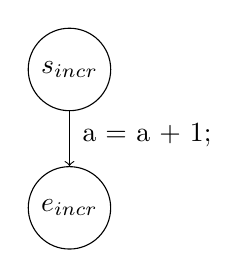
\begin{tikzpicture}[node distance={50pt}, main/.style = {draw, circle}] 
          \node[main] (0) {$s_{incr}$};
          \node[main] (1) [below of=0] {$e_{incr}$};
          \draw[->] (0) -- node[midway, xshift=28pt, yshift=11pt, pos=1] {a = a + 1;} (1);
        \end{tikzpicture}
      \end{subfigure}
      \caption{Example program (left) and corresponding CFGs for \texttt{main} (middle) and \texttt{incr} (right). The asserts in \autoref{code:assert_a} and \autoref{code:assert_c} are proven with a context-sensitive values-of-variables analysis. However, a context-insensitive values-of-variables analysis fails to prove both.}
      \label{fig:example_ctx_sens}
    \end{figure}

  \section{Partial context-sensitivity}\label{sec:partialCtxSens}
    While the context-sensitive approach from the previous section might be very precise, it can be quite costly in terms of computation time. To reach a middle ground between a context-insensitive and a fully context-sensitive analysis, we change the approach so that contexts are different from the entry state of a call. With this we can group entry states by contexts to analyze a procedure multiple times. This time we group not once per individual entry state, but once per group of entry states.\\
    Thus, we now lift the limitation that $\mathbb{C} = \mathbb{D}$. This allows for differentiating function calls not by the entry state but by something different defined by the analysis.\\
    To compute the context when entering a procedure, we define a new function $\textsf{context}^{\#}: \mathbb{D} \rightarrow \mathbb{C}$. Additionally, the constraints for $\textsf{enter}^{\#}$ and $\textsf{combine}^{\#}$ are changed as follows:
    \[\eta\ [s_f, \textsf{context}^{\#}\ (\eta\ [u, c])] \sqsupseteq \textsf{enter}^{\#}\ (\eta\ [u, c]) \]
    \[\eta\ [v, c] \sqsupseteq \textsf{combine}^{\#}\ ((\eta\ [u, c]), (\eta\ [e_f, \textsf{context}^{\#}\ (\eta\ [u, c])])) \]
    for an edge $(u, f();, v)$.\\
    This formalization results in multiple constraints for a single contextualized starting variable $[s_f, c']$. We can alternatively formulate this as
    \[\eta\ [s_f, c'] \sqsupseteq \bigsqcup \{\textsf{enter}^{\#}\ (\eta\ [u_n, c_n]) | \exists (u_n, f();, v_n) \in Edges:\ \textsf{context}^{\#}\ (\eta\ [u_n, c_n]) = c' \} \]
    i.e., the constraint for the variable $[s_f, c']$ is the least upper bound of all entry states for some call of $f$, which have the same context $c'$ as the constraint variable. Or expressed differently, all states computed by $\textsf{enter}^{\#}\ d$ for $f$ are grouped by the context $c' = \textsf{context}^{\#}\ d$, where each group is joined by $\bigsqcup$ to produce a constraint for a starting variable $[s_f, c']$ with the respective context.\\ 
    With this formal model, we have the option to perform an analysis completely context-sensitively ($\mathbb{C} = \mathbb{D}$ and $\textsf{context}^{\#} = \textsf{enter}^{\#}$), completely context-insensitively ($\mathbb{C} = \{\bullet\}$) or anything in between. Note that we define $\{\bullet\}$ as the "unit domain" which contains exactly one element with the trivial ordering $\bullet \sqsubseteq \bullet$.\\
    \\
    We have to note here that there are some severe issues with the approach for (partially) context-sensitive analyses described in this thesis: The resulting system of constraints may not be finite and some variables in the constraint system may depend on an infinite number of other variables. Thus, it is computationally complex to compute a solution to the system of constraints. For simplicity, we stick with the described methodology in the scope of this thesis.\\
    An extension to the approach which addresses the mentioned issue can be found in \parencite{apinis2012side}.

  \section{Precision loss}\label{sec:precisionLoss}
    The main source of the precision loss in context-insensitive or partially context-sensitive analyses is the join over all states with the same context, i.e., when we take the least upper bound of a group of entry states. Consider a procedure $f$ that has no effect, i.e., $s_f = e_f$. Even for this procedure, the $\textsf{combine}^{\#}$ function receives the less precise result of the join $\bigsqcup$ to combine it with the caller state. In this simple case, the result would be more precise if the $\textsf{combine}^{\#}$ function could directly use the result from the corresponding $\textsf{enter}^{\#}$ as the callee state for combining.\\
    Even for procedures that do change the state, there might be some parts of the state which are untouched by the call. If we can identify these untouched parts, we could reduce the precision loss experienced by using partial contexts.\\
    \\
    We clarify the source of the precision loss mentioned above with an example: For this, we once again consider the example program \autoref{fig:example_ctx_sens}. This time we take the marked lines into account. When the program is analyzed context-insensitively, not only does the state at the start node for \texttt{incr()} $s_{incr}$ represent two possible values for the global variable \texttt{a}, but also for \texttt{c}. Therefore, the state for this node is
    \[\eta_\textsf{v}\ [s_{incr}, \bullet] = \{a \rightarrow \{-3, 1\}, c \rightarrow \{-10, 10\}\} \]
    Even though the variable \texttt{c} is never changed within \texttt{incr()}, the mapping $c \rightarrow \{-10, 10\}$ is still copied into the caller state when combining the states for node $v_6$. Thus, the information gained by the context-insensitive values-of-variables analysis does not suffice to determine the assertion in \autoref{code:assert_c} to hold. This loss of precision could easily be avoided if we had some idea of which global variables are definitely not changed by a procedure call.


